\documentclass{article}
\usepackage[utf8x]{inputenc}
%\usepackage{a4wide}
\usepackage[magyar]{babel}
\usepackage{times}
\usepackage{graphicx}
\usepackage[top=0.5in, bottom=0.5in]{geometry}
%opening
\author{Milán Unicsovics}
\title{MSc Önálló laboratórium 1}
\date{\today}
\begin{document}
%%%%%%%%%%%%%%%%%%%Szöveg%%%%%%%%%%%%%%%%%%%%%%
\thispagestyle{empty}
\begin{figure}[htp]
\centering
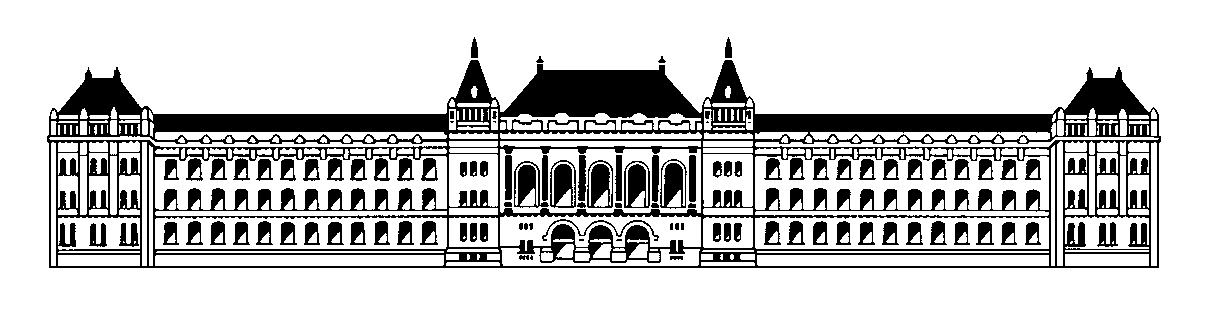
\includegraphics[scale=0.3]{img/bme.png}
\begin{center}
Budapesti Műszaki és Gazdaságtudományi Egyetem\\
Méréstechnika és Információs Rendszerek Tanszék
\end{center}
\end{figure}
\vspace*{-0.1in}
\begin{center}
\subsection*{Tesztgenerálás állapotgép alapú modellekből}
{\bf
Unicsovics Milán György (M9GNTV, I. évf, MSc) mérnök inf. szakos hallgató\\[0.3cm]

Konzulens: Dr. Micskei Zoltán adjunktus, MIT\\[0.3cm]

Szolgáltatásbiztos rendszertervezés szakirány 

Önálló laboratórium 1 összefoglaló 

2013/14. I. félév
}
\end{center}
\vspace{0.5cm}

A tesztelés célja a hibadetektálás, mely során egy szoftver elvárt és aktuális működését összehasonlítjuk. A modell alapú tesztelés ennek egy változata, ahol modellekel írjuk le a tesztelni kívánt szoftver viselkedését. A modellekből tesztek generálhatóak, melyek később futtathatóak a szoftveren. Kutatásaim célja, hogy későbbiekben egy olyan eszköz fejlesztésébe kezdhessek, mely állapotgép alapú modellt használó szoftverekhez tesztelő keretrendszerként használható.

A féléves munkát a tesztelés, bővebben pedig a modell alapú tesztelés megismerésével kezdtem. Ennek során áttekintettem ezen területek alapfogalmait, a modell alapú tesztelés folyamatának részleteit, valamint a használható módszerek egy fajta taxonómiáját is. Az irodalomkutatást az állapotgép alapú modellt használó tesztkeretrendszerek vizsgálatával folytattam, melynek során megismertem konkrét eszközöket a korábbi osztályzásban szereplő különböző módszerekhez. Ezen eszközök összehasonlítása azért is hasznos volt számomra, hiszen olyan tanulságok levonását tette lehetővé, amely a hosszútávú célokhoz nyújthatnak segítséget.

Munkámat két teljesen különböző elvek alapján elkészített tesztkeretrendszer, a PyModel és a GraphWalker tanulmányozásával folytattam. Elsősorban az eszközök használatának munkafolyamatára koncentráltam, figyelmet fordítva a korábban megismert osztályzási szempontokra és a felhasznált technológiákra is. A két eszköz dokumentációinak átolvasása után a gyakorlatban is kipróbáltam ezeket a programokat egy-egy demonstrációs példaalkalmazással.

Érdekes és a féléves munkát meghatározó volt, egy a gráfelméletet a modell alapú teszteléssel összekötő tudományos munka. A cikkben található algoritmusokat (kínai postás problémája, New York-i utcaseprő problémája, de Bruijn szekvenciák keresése, Markov láncok használata véletlenszerű gráfbejárások irányítására) megismertem, először papíron gyakoroltam, később pedig egy implementáció során részletesen is elsajátítottam.

Az olvasott elméleti módszereket és algoritmusokat egy Python nyelven készített teljes körű tesztkeretrendszer fejlesztésével folytattam. Első lépésben egyre összetettebb állapotgépek összeállításába kezdtem, melyeket egy megismert állapotgépleíró formátum az SCXML és az általános gráfleíró adatformátum a GraphML formátumaiban készítettem el. Ezután egy általános felhasználású implementációt készítettem a Python nyelvű matematikai könyvtárak felhasználásával a kínai postás és a New York-i utcaseprő problémák megoldására.

Az általam készített implementáció tehát GraphML formátumban megadott irányítatlan és irányított gráf modellekkel reprezentált szoftverhez tud teljes állapotátmeneti lefedettséget garantáló tesztesetkészletet generálni. A tesztkeretrendszerben adapter és tesztszkript is szerepel, mely a tesztelendő szoftverrel összeköti az állapotgép alapú modellreprezentációt és futtatja a teszteseteket a szoftveren. Végül egy tesztorákulum dönti el, hogy az elvárt kimenet megegyezik-e a tesztesetben szereplő bemenettel.

Az elvégzett feladatok jó bevezetőt nyújtottak a modell alapú tesztelés területére, az elméleti hátteret sikerült áttekinteni a félév során. A megismert módszerek és algoritmusok egy részét sikerült elsajátítani, további céljaim között szerepel ezen ismeretek bővítése és a tapasztaltak gyakorlatban történő demonstrációja. Az adott területhez kapcsolódó szoftverek működéséről is átfogó ismereteket szereztem, melyeket két eszköz gyakorlatban történő kipróbálásával egészítettem ki. Későbbiekben lehetne újabb eszközöket is megismerni. Összesítve elmondhatom, hogy nagyon élveztem a féléves feladatokat és a későbbi munka megalapozását, melyeket következő félévben folytatok.

\end{document}
